\documentclass[11pt,a4paper]{article}

\usepackage[margin=2.25cm]{geometry}
\usepackage{newtxtext,newtxmath}
\usepackage{microtype}
\usepackage{amsmath,mathtools,bm}
\usepackage{siunitx}
\usepackage{booktabs,tabularx,longtable,array}
\usepackage{graphicx}
\graphicspath{{figures/}}
\usepackage{xcolor}
\usepackage{caption}
\usepackage{subcaption}
\usepackage{float}
\usepackage{placeins}
\usepackage{enumitem}
\usepackage{listings}
\usepackage[most]{tcolorbox}
\usepackage{fontawesome5}
\usepackage{tikz}
\usetikzlibrary{arrows.meta,positioning,shapes.geometric,calc}
\usepackage{fancyhdr}
\usepackage[hidelinks]{hyperref}
\usepackage[nameinlink,noabbrev]{cleveref}

\definecolor{NatureBlue}{HTML}{0072B2}
\definecolor{NatureOrange}{HTML}{E69F00}
\definecolor{NatureGreen}{HTML}{009E73}
\definecolor{NatureSky}{HTML}{56B4E9}
\definecolor{NaturePurple}{HTML}{7B61A8}
\definecolor{SoftBlue}{HTML}{EDF6FB}
\definecolor{SoftOrange}{HTML}{FFF5E6}
\definecolor{SoftGreen}{HTML}{ECF8F3}
\definecolor{CodeGrey}{HTML}{F5F5F5}

\hypersetup{
  colorlinks=true,
  linkcolor=NatureBlue,
  citecolor=NatureBlue,
  urlcolor=NatureBlue,
  pdftitle={Propagation-Aware Bragg Transfer-Function Calculator Manual},
  pdfauthor={MIGA programme}
}

\captionsetup{font=small,labelfont=bf,labelsep=period}
\setlength{\parindent}{0pt}
\setlength{\parskip}{0.55em}
\setlist{nosep,leftmargin=1.6em}
\sisetup{detect-all,per-mode=symbol}

\pagestyle{fancy}
\setlength{\headheight}{14pt}
\fancyhf{}
\fancyhead[L]{Propagation-aware Bragg transfer function}
\fancyhead[R]{User and theory manual}
\fancyfoot[C]{\thepage}
\renewcommand{\headrulewidth}{0.4pt}

\newtcolorbox{keybox}[1][Key point]{
  enhanced,colback=SoftBlue,colframe=NatureBlue,boxrule=0.7pt,arc=1.5pt,
  title={\faInfoCircle\quad #1},fonttitle=\bfseries
}
\newtcolorbox{warningbox}[1][Important limitation]{
  enhanced,colback=SoftOrange,colframe=NatureOrange,boxrule=0.7pt,arc=1.5pt,
  title={\faExclamationTriangle\quad #1},fonttitle=\bfseries
}
\newtcolorbox{checkbox}[1][Validation]{
  enhanced,colback=SoftGreen,colframe=NatureGreen,boxrule=0.7pt,arc=1.5pt,
  title={\faCheckCircle\quad #1},fonttitle=\bfseries
}

\lstdefinestyle{manualcode}{
  backgroundcolor=\color{CodeGrey},basicstyle=\ttfamily\small,frame=single,
  rulecolor=\color{black!25},breaklines=true,columns=fullflexible,
  keepspaces=true,showstringspaces=false,keywordstyle=\color{NatureBlue}\bfseries,
  commentstyle=\color{NatureGreen!70!black}
}
\lstset{style=manualcode}

\newcommand{\dd}{\,\mathrm{d}}
\newcommand{\ii}{\mathrm{i}}
\newcommand{\Hatom}{H_{\mathrm{AI}}}
\newcommand{\Hsrc}{H_{\mathrm{src}\phi}}
\newcommand{\Hnu}{H_{\nu}}
\newcommand{\taud}{\tau_{d}}
\newcommand{\Oraw}{\Omega_{\mathrm{raw}}}
\newcommand{\Oeff}{\Omega_{\mathrm{eff}}}
\newcommand{\CaseDelayUs}{1.000692}
\newcommand{\CaseHalfOverlapUs}{23.999308}
\newcommand{\CasePiOverlapUs}{48.999308}
\newcommand{\CaseHalfAreaRatio}{0.959972}
\newcommand{\CasePiAreaRatio}{0.979986}
\newcommand{\CaseHalfScale}{1.041697}
\newcommand{\CasePiScale}{1.020423}
\newcommand{\CaseHalfPeakA}{10.4170}
\newcommand{\CasePiPeakA}{10.2042}
\newcommand{\CaseContrastB}{0.990143}
\newcommand{\CaseHZeroTenK}{2.054095}
\newcommand{\CaseHATenK}{2.070906}
\newcommand{\CaseHBTenK}{2.066469}
\newcommand{\CaseHAHundredK}{1.420195e-01}
\newcommand{\CaseHBHundredK}{1.463735e-01}
\newcommand{\CaseDTenK}{0.062865}
\newcommand{\CaseDHundredK}{0.618448}


\title{\vspace{-1.3cm}\textbf{Propagation-Aware Bragg Transfer-Function Calculator}\\[0.35em]
\large Theory, numerical implementation and worked \SI{150}{\metre} case}
\author{MIGA programme}
\date{Version 1.0 \textbullet{} 1 September 2026}

\begin{document}

\maketitle
\begin{center}\rule{0.92\textwidth}{0.6pt}\end{center}

\begin{abstract}
This manual documents \texttt{bragg\_transfer\_function\_propagation\_ui.py}, a propagation-aware extension of the finite-pulse Bragg transfer-function calculator. In a single-frequency retroreflected geometry, the two fields seen by an atom carry optical envelopes separated by the round-trip time $\taud=2L/c$. Their incomplete temporal overlap changes the effective two-photon Rabi envelope and, if the pulse is not recalibrated, its area. The program implements two complementary limits: Model A restores every nominal pulse area after the overlap loss, whereas Model B keeps the incident setting fixed and propagates the resulting nonideal two-level rotations. The manual derives both models, distinguishes the atomic, delay and combined transfer functions, documents the numerical procedure and interface, and presents a reproducible first-order square-pulse example for $L=\SI{150}{\metre}$, $\tau_{\pi}=\SI{50}{\micro\second}$ and $\tau_{\pi/2}=\SI{25}{\micro\second}$.
\end{abstract}

\begin{keybox}[The central distinction]
$\Hatom$ maps the \emph{local counter-propagating Bragg phase} at the atoms to interferometer phase and is dimensionless. The propagation factor $D_d$ maps source phase to that local phase difference and is also dimensionless. Their product $\Hsrc=\Hatom D_d$ maps source phase to atom phase. Only after converting source frequency noise in hertz into phase does one obtain $\Hnu=\Hsrc/(\ii f)$, whose unit is rad/Hz.
\end{keybox}

\tableofcontents
\clearpage

\section{Purpose and model boundary}

The calculator describes a resonant three-pulse Mach--Zehnder sequence with nominal areas $\pi/2$--$\pi$--$\pi/2$. It extends the sensitivity-function treatment of finite laser pulses used by Cheinet \textit{et al.}\cite{Cheinet2008}, the MIGA phase-noise analysis\cite{Canuel2018}, and pulse-shaping calculations based on the time-dependent pulse area\cite{Fang2018}. The extension considered here is deliberately specific: a forward pulse envelope and its retroreflected copy arrive at the atoms at different times.

The dynamics backend is an effective resonant two-level model. The Bragg order $n$ is an external phase-gain multiplier. The software therefore captures propagation-induced envelope overlap, pulse-area loss, finite-pulse filtering and laser phase/frequency-noise conversion, but it does not predict the momentum-state ladder, velocity selectivity, diffraction phase, AC Stark shift, Doppler detuning, spontaneous emission, parasitic interferometers or optical-cavity dynamics. Those effects require a multi-state Bragg Hamiltonian such as the treatments discussed in Refs.~\cite{Siemss2020,Jenewein2022}.

\begin{figure}[H]
\centering
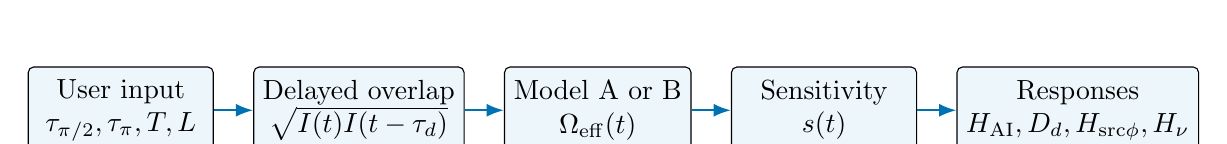
\begin{tikzpicture}[
  node distance=6mm and 5mm,
  block/.style={draw,rounded corners=2pt,minimum width=2.35cm,minimum height=1.1cm,align=center,fill=SoftBlue},
  arrow/.style={-{Latex[length=2.2mm]},thick,NatureBlue}
]
\node[block] (input) {User input\\$\tau_{\pi/2},\tau_\pi,T,L$};
\node[block,right=of input] (overlap) {Delayed overlap\\$\sqrt{I(t)I(t-\taud)}$};
\node[block,right=of overlap] (model) {Model A or B\\$\Oeff(t)$};
\node[block,right=of model] (sens) {Sensitivity\\$s(t)$};
\node[block,right=of sens] (out) {Responses\\$\Hatom,D_d,\Hsrc,\Hnu$};
\draw[arrow] (input)--(overlap);
\draw[arrow] (overlap)--(model);
\draw[arrow] (model)--(sens);
\draw[arrow] (sens)--(out);
\end{tikzpicture}
\caption{Calculation chain. Propagation first changes the local Rabi envelope; the chosen pulse-area model then determines the sensitivity function and the atomic response. A separate delay filter converts source laser noise into the local counter-propagating phase.}
\label{fig:workflow}
\end{figure}

\section{Quick start}

From the project directory, launch the graphical interface with

\begin{lstlisting}[language=bash]
python3 bragg_transfer_function_propagation_ui.py
\end{lstlisting}

Run the built-in consistency checks with

\begin{lstlisting}[language=bash]
python3 bragg_transfer_function_propagation_ui.py --self-test
\end{lstlisting}

The input widths are always entered in microseconds. For a square pulse they are its command durations; for a Gaussian they are optical-intensity FWHM values. The program converts them to the nominal peak two-photon Rabi rates required to obtain the target areas before propagation is applied. The pulse separation $T$ is centre-to-centre for both pulse shapes. The mirror distance $L$ is the one-way atom-to-retroreflector distance.

The recommended workflow is to calculate Model A and Model B with the same inputs. Model A answers ``what remains after the experimenter recalibrates each pulse area?'' Model B answers ``what happens if the original pulse setting is left unchanged?'' Neither model is universally more correct; they represent different experimental control assumptions.

\section{Geometry and propagation delay}

Let the source-side phase and intensity envelope be $\phi(t)$ and $I(t)$. At the atoms, choose the forward field as the time reference. The retroreflected field contains an earlier source sample delayed by the round-trip propagation time
\begin{equation}
  \taud=\frac{2L}{c}.
  \label{eq:delay}
\end{equation}
Ignoring constant propagation phases and using a common spatial mode, the complex two-photon coupling can be written
\begin{equation}
  \widetilde{\Omega}(t)=\Omega_{\mathrm{in}}
  \frac{\sqrt{I(t)I(t-\taud)}}{I_{\mathrm{pk}}}
  \exp\!\left\{\ii[\phi(t)-\phi(t-\taud)]\right\}.
  \label{eq:complex-rabi}
\end{equation}
The modulus of \cref{eq:complex-rabi} gives the raw Rabi envelope used to construct the pulses,
\begin{equation}
  \Oraw(t)=\Omega_{\mathrm{in}}
  \frac{\sqrt{I(t)I(t-\taud)}}{I_{\mathrm{pk}}},
  \label{eq:raw-rabi}
\end{equation}
whereas the argument gives the local phase difference that drives the interferometer. These two propagation effects must not be conflated: envelope overlap modifies $s(t)$ and hence $\Hatom$; phase differencing supplies the independent factor $D_d$ introduced in \cref{sec:transfer}.

\begin{warningbox}[Definition of $L$]
The software uses $\taud=2L/c$. Entering an optical path length that already includes the round trip would count the factor of two twice. Any additional fibre, free-space or electronic delay must be added explicitly if it is part of the physical comparison.
\end{warningbox}

\section{Effective pulse envelopes}

\subsection{Square pulses}

For a square command of duration $\tau$ centred on $t_c$, the two unit-height envelopes overlap for
\begin{equation}
  \tau_{\mathrm{ov}}=\tau-\taud,
  \qquad \tau>\taud,
  \label{eq:square-overlap}
\end{equation}
and the overlap is centred at $t_c+\taud/2$. The raw Rabi rate is unchanged inside that shorter interval, so
\begin{equation}
  A_{\mathrm{raw}}=\int\Oraw(t)\dd t
  =\Omega_{\mathrm{in}}(\tau-\taud),
  \qquad
  \frac{A_{\mathrm{raw}}}{A_0}=1-\frac{\taud}{\tau}.
  \label{eq:square-area}
\end{equation}
If $\taud\geq\tau$, the two envelopes do not overlap and the code stops with an explanatory error rather than returning a fictitious pulse.

\subsection{Gaussian pulses}

The Gaussian input convention is
\begin{equation}
 I(t)=I_{\mathrm{pk}}\exp\!\left[-\frac{(t-t_c)^2}{2\sigma^2}\right],
 \qquad \tau_{\mathrm{FWHM}}=2\sqrt{2\ln2}\,\sigma.
\end{equation}
Taking the geometric mean in \cref{eq:raw-rabi} gives
\begin{equation}
 \Oraw(t)=\Omega_{\mathrm{in}}
 \exp\!\left[-\frac{\taud^2}{8\sigma^2}\right]
 \exp\!\left[-\frac{(t-t_c-\taud/2)^2}{2\sigma^2}\right].
 \label{eq:gaussian-overlap}
\end{equation}
Thus an untruncated Gaussian keeps the same $\sigma$ and shifts by $\taud/2$. Its peak is attenuated by the first exponential in \cref{eq:gaussian-overlap}. Numerically, the program truncates each input at $\pm6\sigma$; the common support and its error-function area are retained exactly when constructing the pulse.

\section{Two propagation models}

\subsection{Model A: area compensated}

Model A multiplies every raw envelope by
\begin{equation}
  \alpha_j=\frac{A_j^{\mathrm{target}}}{A_j^{\mathrm{raw}}},
  \qquad
  {\Oeff}_j(t)=\alpha_j{\Oraw}_j(t),
  \label{eq:model-a}
\end{equation}
where $A_j^{\mathrm{target}}\in\{\pi/2,\pi,\pi/2\}$. It represents an experiment in which the delayed pulse is recalibrated by increasing optical power or Rabi rate. Propagation can still change the pulse duration, centre and spectral envelope, even though the integrated areas are ideal.

For ideal pulse areas, define the accumulated pulse area
\begin{equation}
  \Theta_j(t)=\int_{t_{j,\mathrm{s}}}^{t}{\Oeff}_j(t')\dd t'.
\end{equation}
The usual MIGA/Cheinet sign convention gives the sensitivity function
\begin{equation}
s_A(t)=
\begin{cases}
 \sin\Theta_1(t), & t\text{ in the first }\pi/2\text{ pulse},\\
 +1, & \text{between pulses 1 and 2},\\
 \cos\Theta_2(t), & t\text{ in the }\pi\text{ pulse},\\
 -1, & \text{between pulses 2 and 3},\\
 -\cos\Theta_3(t), & t\text{ in the last }\pi/2\text{ pulse},\\
 0, & \text{otherwise}.
\end{cases}
\label{eq:ideal-sensitivity}
\end{equation}
The code evaluates the same physical response through the common two-level phase-step routine, ensuring that Models A and B use one sign and timing convention.

\subsection{Model B: fixed input}

Model B sets $\alpha_j=1$. The areas are generally not exactly $\pi/2$, $\pi$ and $\pi/2$, so inserting them into the ideal piecewise formula would be inconsistent. Instead, the program propagates the resonant two-level state with the rotation
\begin{equation}
 R(A,\varphi)=
 \begin{pmatrix}
  \cos(A/2)&-\ii e^{-\ii\varphi}\sin(A/2)\\
  -\ii e^{\ii\varphi}\sin(A/2)&\cos(A/2)
 \end{pmatrix}.
 \label{eq:rotation}
\end{equation}
To evaluate the sensitivity at time $t$, an infinitesimal phase step $\epsilon$ is inserted: the part of the active pulse before $t$ uses phase $\varphi$, and all subsequent evolution uses $\varphi+\epsilon$. A symmetric finite difference gives $\partial P/\partial\epsilon$. The result is normalized by the output fringe slope at the operating point,
\begin{equation}
 s_B(t)=-\frac{\partial P(t)/\partial\epsilon}
 {\partial P/\partial\varphi_{3}},
 \label{eq:model-b-sensitivity}
\end{equation}
where the minus sign enforces the convention that the first plateau is positive. This normalization expresses the response as inferred atom phase. If the fringe slope becomes nearly zero, that inferred phase is ill-conditioned; the program reports an error.

\begin{keybox}[What Model B includes]
Model B includes reduced pulse area and fringe contrast within a resonant effective two-level system. It does not turn the calculation into a full Bragg diffraction simulation. In particular, loss into unwanted momentum orders and diffraction phase are absent.
\end{keybox}

\section{Sensitivity and transfer functions}\label{sec:transfer}

The Fourier convention used throughout is
\begin{equation}
 \mathcal{F}[x](\omega)=\int_{-\infty}^{\infty}x(t)e^{-\ii\omega t}\dd t,
 \qquad \omega=2\pi f.
 \label{eq:fourier}
\end{equation}
The atomic phase response to the local Bragg phase is
\begin{equation}
 \Hatom(f)=n\int_{-\infty}^{\infty}\dot{s}(t)e^{-\ii2\pi ft}\dd t
 =n\,\ii2\pi f\int_{-\infty}^{\infty}s(t)e^{-\ii2\pi ft}\dd t.
 \label{eq:hai}
\end{equation}
The second equality follows by integration by parts because $s(t)$ vanishes outside the interferometer sequence. This is the same integral written in two numerically equivalent ways; the code uses the right-hand form because $s(t)$ is smooth inside each pulse and constant during free evolution. At $f=0$, $\Hatom(0)=0$.

The local counter-propagating phase in \cref{eq:complex-rabi} is $\phi(t)-\phi(t-\taud)$. Its frequency-domain filter is therefore
\begin{equation}
 D_d(f)=1-e^{-\ii2\pi f\taud}
 =2\ii e^{-\ii\pi f\taud}\sin(\pi f\taud),
 \qquad |D_d|=2|\sin(\pi f\taud)|.
 \label{eq:delay-filter}
\end{equation}
The total response to source laser phase is
\begin{equation}
 \Hsrc(f)=\Hatom(f)D_d(f).
 \label{eq:hsrc}
\end{equation}
If frequency noise is specified as $\delta\nu(f)$ in hertz, then $\delta\phi(f)=\delta\nu(f)/(\ii f)$ under the convention of \cref{eq:fourier}. Consequently,
\begin{equation}
 \Hnu(f)=\frac{\Hsrc(f)}{\ii f}.
 \label{eq:hnu}
\end{equation}
The apparent missing $2\pi$ is intentional: $\dot\phi=2\pi\delta\nu$ and the angular Fourier denominator is $\ii2\pi f$, so the factors cancel.

\begin{table}[H]
\centering
\caption{Meaning and units of the four displayed responses.}
\label{tab:units}
\begin{tabularx}{\textwidth}{@{}lllX@{}}
\toprule
Quantity & Input $\rightarrow$ output & Unit & Interpretation \\
\midrule
$\Hatom$ & local Bragg phase $\rightarrow$ atom phase & dimensionless & Atomic sequence and finite-pulse filtering \\
$D_d$ & source phase $\rightarrow$ local phase difference & dimensionless & Pure round-trip delay differencer \\
$\Hsrc$ & source phase $\rightarrow$ atom phase & dimensionless & Product $\Hatom D_d$ \\
$\Hnu$ & source frequency in Hz $\rightarrow$ atom phase & rad/Hz & Product $\Hsrc/(\ii f)$ \\
\bottomrule
\end{tabularx}
\end{table}

For a one-sided input power spectral density $S_x(f)$, the output is
\begin{equation}
 S_{\Phi}(f)=|H_x(f)|^2S_x(f),
 \qquad
 \sigma_\Phi^2=\int_0^\infty S_\Phi(f)\dd f.
 \label{eq:psd}
\end{equation}
For amplitude spectral densities, use $\sqrt{S_\Phi}=|H_x|\sqrt{S_x}$. Do not multiply an ASD by $|H|^2$.

\section{Numerical implementation}

The schedule builder first converts the entered widths to nominal peak Rabi rates. For square pulses, $\Omega_{\pi/2}=(\pi/2)/\tau_{\pi/2}$ and $\Omega_\pi=\pi/\tau_\pi$. For Gaussian pulses, the same target areas are divided by the truncated Gaussian integral. Each delayed effective pulse then stores its support, shifted centre, raw and effective areas, raw and compensated peak rates, and the cumulative-area function.

The transfer-function routine computes $\int s(t)e^{-\ii\omega t}\dd t$. Inside pulses, Gauss--Legendre quadrature samples the phase-step sensitivity. The long constant plateaus are integrated analytically with the stable identity
\begin{equation}
 \int_0^d e^{\ii q t}\dd t
 =d\,e^{\ii qd/2}\operatorname{sinc}\!\left(\frac{qd}{2}\right),
 \qquad \operatorname{sinc}(x)=\frac{\sin x}{x}.
 \label{eq:stable-integral}
\end{equation}
NumPy defines \texttt{sinc(x)} as $\sin(\pi x)/(\pi x)$, so the implementation passes $qd/(2\pi)$. This avoids the removable singularity at $q=0$. Frequencies are processed in chunks to limit memory use. The quadrature order grows with the product of maximum frequency and pulse duration and is capped at 4096 nodes so that an unreasonable request fails transparently.

\begin{checkbox}[Internal checks]
The command-line self-test verifies the zero-delay limit, the square overlap formula, Model A area restoration, Model B area loss, the analytic delay factor and the relationship $\Hsrc=\Hatom D_d$. It also checks that $\Hnu=\Hsrc/(\ii f)$ away from DC.
\end{checkbox}

\section{Graphical interface and plot reading}

The interface accepts Bragg order, $\pi/2$ and $\pi$ widths in microseconds, centre separation $T$, mirror distance $L$, pulse shape, propagation model and frequency grid. Its panels separate the calculation into physical layers: pulse overlap and effective Rabi envelope; sensitivity function; atomic response; delay filter; combined source-phase response; and frequency-noise response. Saving as PDF or SVG preserves vector curves.

Rapid fringes in $|\Hatom|$ arise from the long separation $T$, while the broad high-frequency roll-off is controlled by the finite pulse widths. A curve evaluated at a single frequency can land arbitrarily close to an interference zero. For envelope comparisons in this manual, the plotted ``local RMS'' averages $|H|^2$ over a small neighbourhood before taking the square root. It is a visualization aid, not a different transfer function and not a physical noise integration bandwidth.

\section{Worked case: \texorpdfstring{$L=\SI{150}{\metre}$}{L=150 m}}\label{sec:case}

\subsection{Inputs and immediate consequences}

The reproducible case uses first-order Bragg diffraction, square pulses, $\tau_{\pi/2}=\SI{25}{\micro\second}$, $\tau_\pi=\SI{50}{\micro\second}$ and $T=\SI{250}{\milli\second}$. Both nominal Rabi rates are therefore $\Omega/(2\pi)=\SI{10}{\kilo\hertz}$. The frequency plots cover \SI{0.1}{\hertz}--\SI{100}{\kilo\hertz}.

\begin{table}[H]
\centering
\caption{Propagation quantities calculated directly from the case inputs.}
\label{tab:case-values}
\begin{tabularx}{\textwidth}{@{}lcccX@{}}
\toprule
Quantity & No delay & Model A & Model B & Meaning \\
\midrule
Round-trip delay $\taud$ ($\si{\micro\second}$) & 0 & \CaseDelayUs & \CaseDelayUs & $2L/c$ \\
$\pi/2$ effective duration ($\si{\micro\second}$) & 25 & \CaseHalfOverlapUs & \CaseHalfOverlapUs & $25-\taud$ \\
$\pi$ effective duration ($\si{\micro\second}$) & 50 & \CasePiOverlapUs & \CasePiOverlapUs & $50-\taud$ \\
$\pi/2$ area / target area & 1 & 1 & \CaseHalfAreaRatio & fixed-input loss \\
$\pi$ area / target area & 1 & 1 & \CasePiAreaRatio & fixed-input loss \\
$\pi/2$ compensation $\alpha$ & 1 & \CaseHalfScale & 1 & Rabi-rate multiplier \\
$\pi$ compensation $\alpha$ & 1 & \CasePiScale & 1 & Rabi-rate multiplier \\
Fringe contrast & 1 & 1 & \CaseContrastB & two-level Model B \\
\bottomrule
\end{tabularx}
\end{table}

The delay is \SI{\CaseDelayUs}{\micro\second}, about 4.00\% of a $\pi/2$ command and 2.00\% of a $\pi$ command. Model A restores the areas by raising the effective peaks from \SI{10}{\kilo\hertz} to \SI{\CaseHalfPeakA}{\kilo\hertz} and \SI{\CasePiPeakA}{\kilo\hertz}, respectively. Model B retains the \SI{10}{\kilo\hertz} peak and loses the same fractions of area. Its predicted contrast remains high, \CaseContrastB, but is not exactly unity.

\begin{figure}[H]
\centering
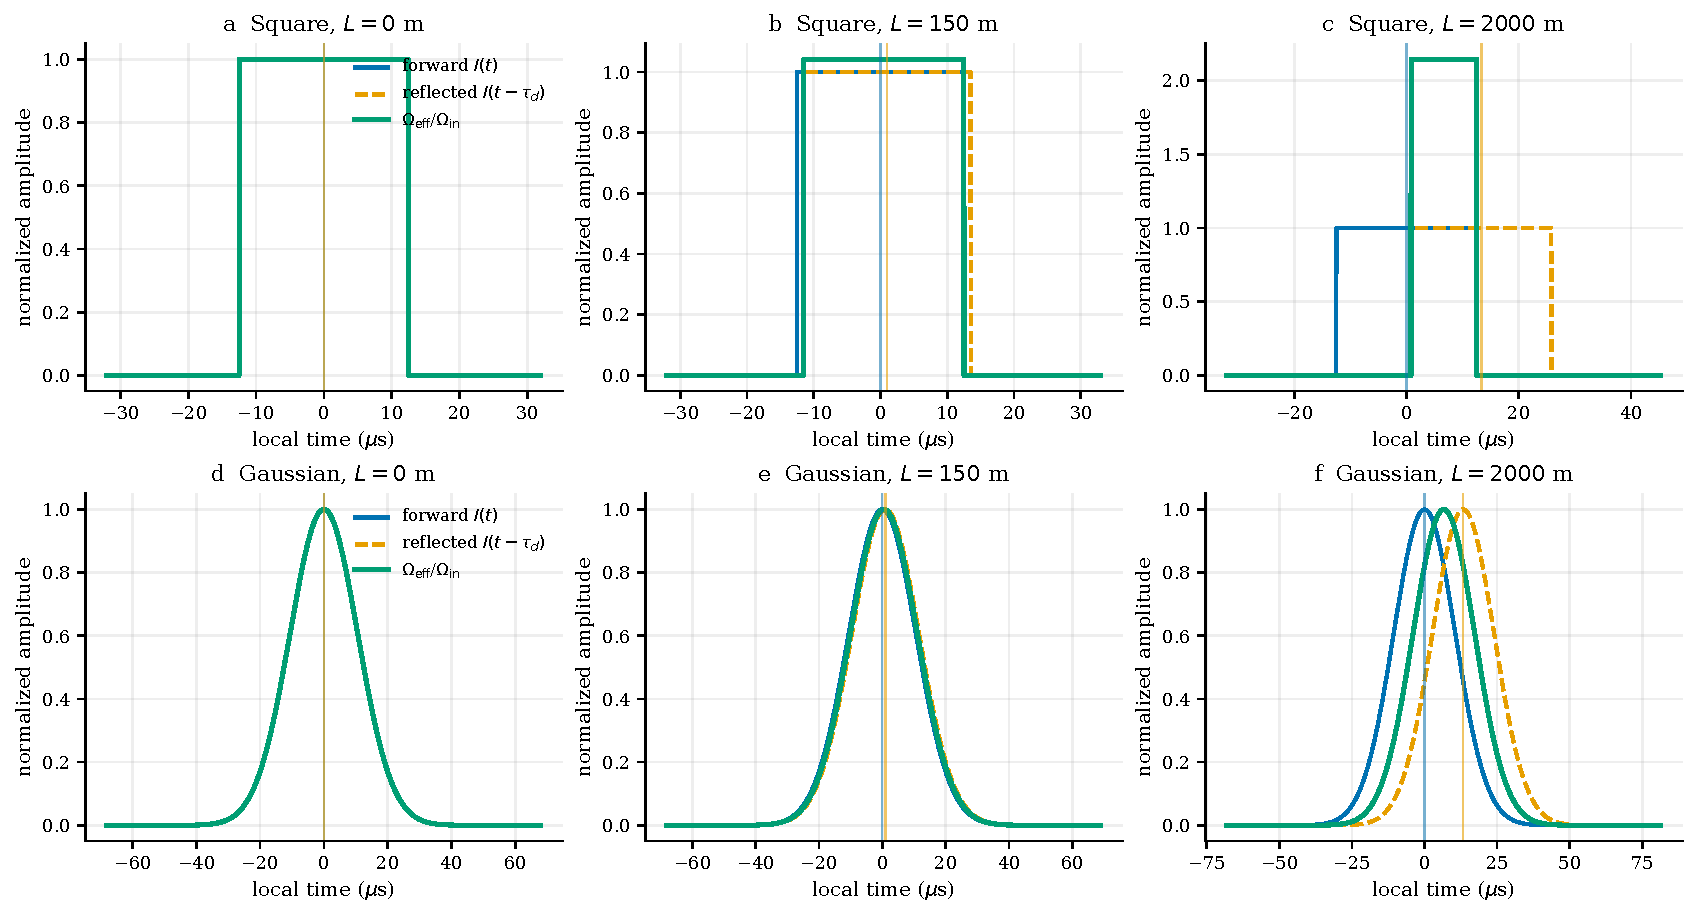
\includegraphics[width=\textwidth]{case_overlap_sensitivity.pdf}
\caption{Delayed overlap and sensitivity function for the \SI{150}{\metre} case. (a) The reflected square envelope is shifted by $\taud$, leaving only the green common interval. (b) Model B retains the nominal peak over a shorter interval; Model A compensates the area with a larger peak. (c) The full sensitivity functions are visually close because $\taud\ll T$, although their pulse-edge details differ. Blue shading marks the effective interaction windows.}
\label{fig:case-overlap}
\end{figure}

\subsection{Change of the atomic response}

At frequencies of order $1/T$, propagation has almost no visible influence on $\Hatom$: it changes microsecond pulse edges while the free evolution lasts hundreds of milliseconds. The low-frequency fringe positions therefore remain governed by $T$. The change becomes clearer near and above the nominal Rabi rate, where the pulse-edge Fourier content is important. Model A has shorter, slightly stronger rotations; Model B has shorter, under-area rotations and a small contrast reduction.

\begin{figure}[H]
\centering
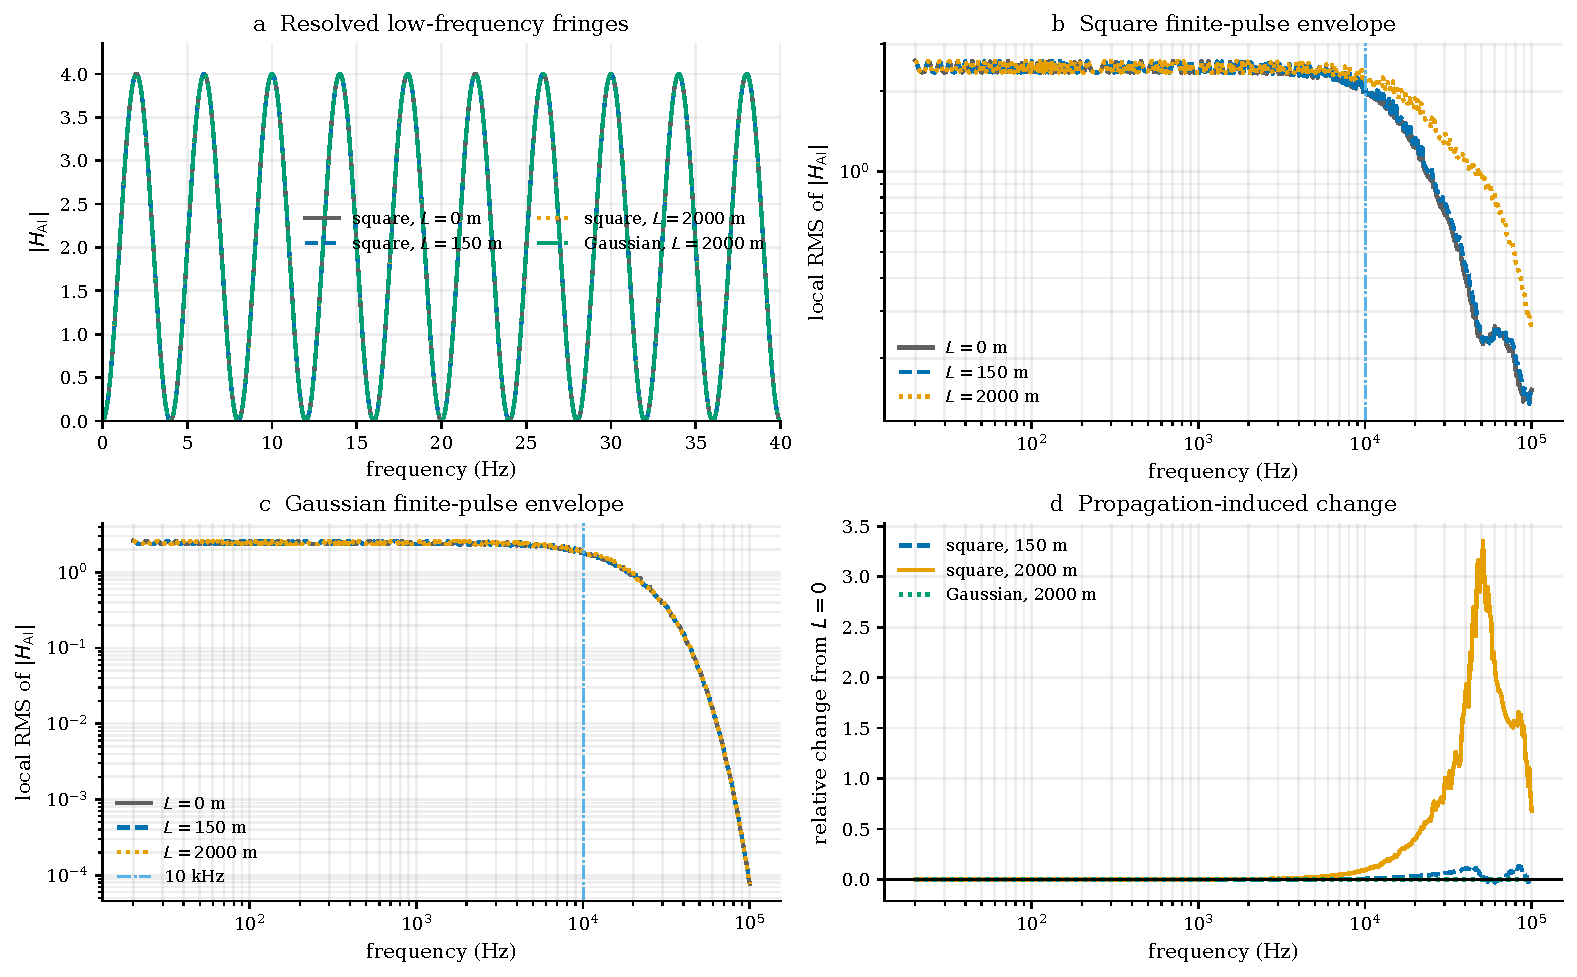
\includegraphics[width=\textwidth]{case_atomic_transfer.pdf}
\caption{Atomic transfer function for the case. (a) Resolved low-frequency fringes are almost indistinguishable. (b) A local RMS reveals the finite-pulse envelope up to \SI{100}{\kilo\hertz}. (c) Relative changes grow near high-frequency lobes and zeros. Ratios near a zero of the no-delay response must be interpreted cautiously because a small displacement of the zero can produce a large ratio.}
\label{fig:case-atomic}
\end{figure}

For a quantitative but zero-insensitive comparison, a $\pm\SI{2}{\hertz}$ local RMS gives the values in \cref{tab:transfer-case}. This window averages several neighbouring samples only; the underlying code always returns the complex pointwise transfer function.

\begin{table}[H]
\centering
\caption{Selected local-RMS atomic responses and delay factors.}
\label{tab:transfer-case}
\begin{tabular}{@{}lccc@{}}
\toprule
Frequency & No-delay $|\Hatom|$ & Model A $|\Hatom|$ & Model B $|\Hatom|$ \\
\midrule
\SI{10}{\kilo\hertz} & \CaseHZeroTenK & \CaseHATenK & \CaseHBTenK \\
\SI{100}{\kilo\hertz} & --- & \CaseHAHundredK & \CaseHBHundredK \\
\bottomrule
\end{tabular}
\qquad
\begin{tabular}{@{}lc@{}}
\toprule
Frequency & $|D_d|$ \\
\midrule
\SI{10}{\kilo\hertz} & \CaseDTenK \\
\SI{100}{\kilo\hertz} & \CaseDHundredK \\
\bottomrule
\end{tabular}
\end{table}

\subsection{Propagation filter and total response}

For this distance, the first exact zero of $D_d$ above DC is $1/\taud\simeq\SI{999.3}{\kilo\hertz}$, outside the plotted range. Below that zero, $|D_d|$ grows approximately as $2\pi f\taud$. Thus the source-phase response is much smaller than the local-phase atomic response at low frequency, not because the atom interferometer has changed units, but because common source phase is rejected by two nearly simultaneous optical samples.

\begin{figure}[H]
\centering
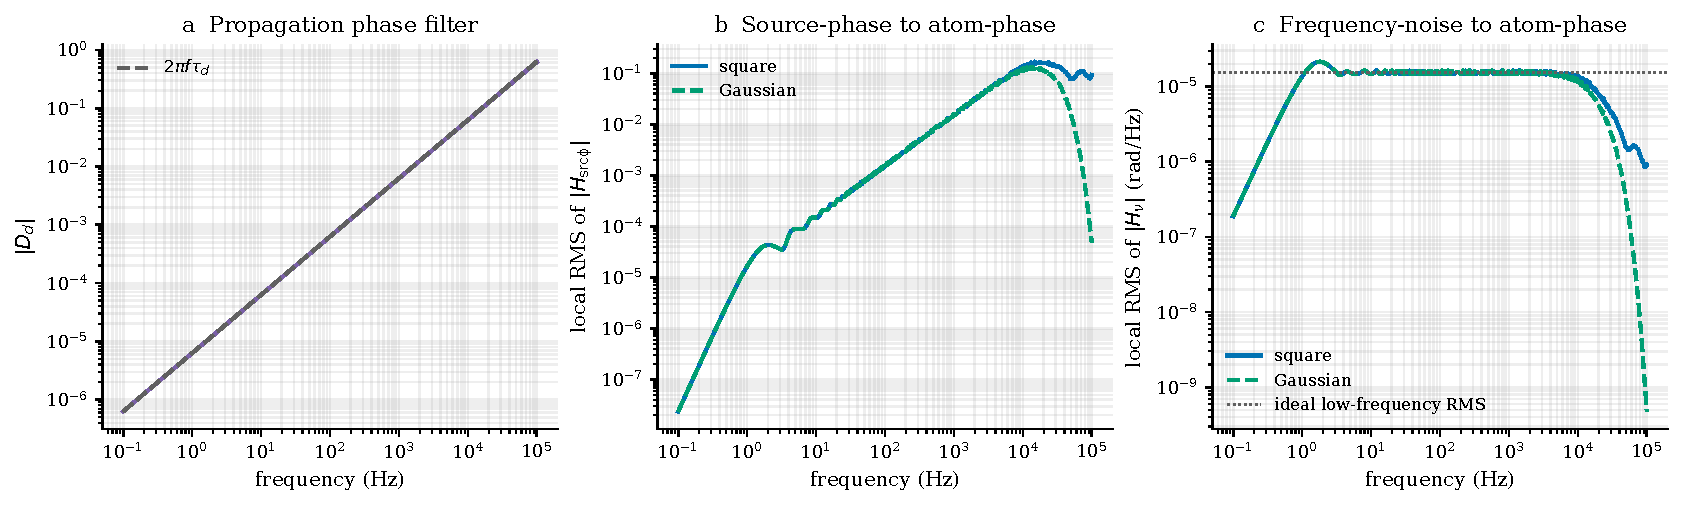
\includegraphics[width=\textwidth]{case_total_transfer.pdf}
\caption{Propagation and combined responses. (a) Exact delay filter and its low-frequency approximation. (b) Combined source-phase response $|\Hsrc|=|\Hatom D_d|$. (c) Source-frequency-noise response $|\Hnu|=|\Hsrc|/f$ in rad/Hz. The dotted low-frequency level is the ideal-pulse local-RMS limit $2\pi\taud\sqrt{6}$ for $n=1$ and the present RMS convention.}
\label{fig:case-total}
\end{figure}

At \SI{10}{\kilo\hertz}, the delay factor is only \CaseDTenK; at \SI{100}{\kilo\hertz} it reaches \CaseDHundredK. The total transfer is the pointwise complex product, so its phase as well as its magnitude must be retained when combining several noise paths. Model A and Model B remain close in this example because the delay occupies only a few percent of each pulse, but their difference would increase for shorter pulses, larger $L$, or a sequence operated near a fringe-slope minimum.

\begin{keybox}[Case conclusion]
For $L=\SI{150}{\metre}$ and 25/\SI{50}{\micro\second} square pulses, propagation has a modest effect on $\Hatom$ itself and a much more conspicuous effect through the source-phase differencer $D_d$. The distinction is experimentally important: calibrating the pulse area addresses the envelope-overlap effect (Model A), but it cannot remove the delayed sampling of source phase.
\end{keybox}

\section{Reproducing the case figures}

The manual directory contains a deterministic plotting script. From that directory run
\begin{lstlisting}[language=bash]
python3 manual_figures_propagation.py
pdflatex -interaction=nonstopmode bragg_transfer_function_propagation_manual.tex
pdflatex -interaction=nonstopmode bragg_transfer_function_propagation_manual.tex
\end{lstlisting}
The script imports the same calculation functions as the GUI, writes vector PDF and preview PNG figures, and regenerates \texttt{case\_values.tex}. The latter prevents hand-copied numbers in the prose from drifting away from the code. Running \LaTeX{} twice resolves the table of contents and cross-references. The source is compatible with Overleaf when the source file, \texttt{case\_values.tex}, and the \texttt{figures} folder are uploaded together.

\section{Troubleshooting and interpretation}

\begin{longtable}{@{}>{\raggedright\arraybackslash}p{0.27\textwidth}>{\raggedright\arraybackslash}p{0.67\textwidth}@{}}
\toprule
Observation & Explanation and action \\
\midrule
\endhead
No square-pulse overlap & $\taud\geq\tau$ for at least one pulse. Reduce $L$, lengthen the pulse, or use a model that represents a different optical timing protocol. \\
Model B reports a small fringe slope & The chosen nonideal areas place the readout near an insensitive operating point. An inferred phase transfer function is then ill-conditioned; inspect transition probability and retune the sequence. \\
$\Hatom$ has no unit but $\Hnu$ does & They have different inputs. $\Hatom$ is phase/phase; $\Hnu$ is phase/frequency and therefore has unit rad/Hz. \\
Large relative-change spikes & The no-delay denominator is near an interference zero. Compare complex responses or a local envelope instead of relying on a ratio. \\
Model A peak exceeds the nominal value & This is the area-restoring factor in \cref{eq:model-a}. Confirm that the required optical power is experimentally available. \\
Gaussian result differs from a square estimate & Gaussian overlap reduces the peak exponentially rather than simply subtracting a duration; use \cref{eq:gaussian-overlap}. \\
Result disagrees with a multi-order Bragg simulation & The present backend is an effective two-level model. Include the momentum ladder, detuning and diffraction phases before treating the discrepancy as a numerical error. \\
\bottomrule
\end{longtable}

\section{Extensions}

The most useful next extension is to allow distinct phase and group delays. The optical carrier phase difference and pulse-envelope overlap need not experience identical propagation in a dispersive fibre or cavity. A second extension is a full momentum-state Hamiltonian, in which Model B naturally predicts unwanted diffraction orders and diffraction phase. Other practical additions include unequal forward/reflected intensities, mirror motion, frequency-dependent optical transfer, independently timed pulses and measured pulse envelopes imported from data.

\section{File map}

\begin{tabularx}{\textwidth}{@{}lX@{}}
\toprule
File & Role \\
\midrule
\texttt{bragg\_transfer\_function\_propagation\_ui.py} & GUI, pulse construction, two-level sensitivity and all transfer functions. \\
\texttt{PROPAGATION\_MODEL.md} & Concise model definition and launch instructions. \\
\texttt{docs/Bragg transfer function propagation/} & This manual, generated values and reproducible case figures. \\
\texttt{manual\_figures\_propagation.py} & Deterministic generator for the three case figures and numerical macros. \\
\bottomrule
\end{tabularx}

\footnotesize
\begin{thebibliography}{9}
\setlength{\itemsep}{0pt}
\bibitem{Cheinet2008}
P.~Cheinet \textit{et al.}, Measurement of the sensitivity function in a time-domain atomic interferometer, \textit{IEEE Trans. Instrum. Meas.} \textbf{57}, 1141--1148 (2008). \href{https://doi.org/10.1109/TIM.2007.915148}{doi:10.1109/TIM.2007.915148}.

\bibitem{Canuel2018}
B.~Canuel \textit{et al.}, Exploring gravity with the MIGA large scale atom interferometer, \textit{Sci. Rep.} \textbf{8}, 14064 (2018). \href{https://doi.org/10.1038/s41598-018-32165-z}{doi:10.1038/s41598-018-32165-z}.

\bibitem{Fang2018}
B.~Fang \textit{et al.}, Improving the phase response of an atom interferometer by means of temporal pulse shaping, \textit{New J. Phys.} \textbf{20}, 023020 (2018). \href{https://doi.org/10.1088/1367-2630/aaa37c}{doi:10.1088/1367-2630/aaa37c}.

\bibitem{Siemss2020}
J.-N.~Siem\ss{} \textit{et al.}, Analytic theory for Bragg atom interferometry based on the adiabatic theorem, \textit{Phys. Rev. A} \textbf{102}, 033709 (2020). \href{https://doi.org/10.1103/PhysRevA.102.033709}{doi:10.1103/PhysRevA.102.033709}.

\bibitem{Jenewein2022}
J.~Jenewein \textit{et al.}, Multiport atom interferometry with Bragg pulses, \textit{Phys. Rev. A} \textbf{105}, 063316 (2022). \href{https://doi.org/10.1103/PhysRevA.105.063316}{doi:10.1103/PhysRevA.105.063316}.
\end{thebibliography}

\end{document}
